\chapter{Sistemi di supporto alle decisioni}
\label{cap:sistemi-supporto-decisioni}

I Sistemi di Supporto alle Decisioni (DSS) sono strumenti informatici progettati per assistere gli utenti nel processo decisionale, utilizzando dati e modelli per risolvere problemi complessi e non strutturati. Questi sistemi combinano l'uso di dati, modelli analitici e strumenti di supporto interattivi per aiutare a prendere decisioni più informate. I DSS possono essere applicati in vari settori, tra cui il business, la sanità, la finanza e la gestione delle risorse umane.\\
Si suddividono in tre categorie principali:
\begin{itemize}
    \item DSS orientati ai dati: si concentrano sulla raccolta e l'analisi dei dati. Utilizzano database e data warehouse per memorizzare grandi quantità di dati e strumenti di data mining per estrarre informazioni utili.
    \item DSS orientati ai modelli: utilizzano modelli matematici e statistici per analizzare i dati e supportare il processo decisionale. Questi modelli possono includere modelli di ottimizzazione, simulazione, previsione e analisi delle serie temporali.
    \item DSS orientati alla conoscenza: incorporano conoscenze specifiche del dominio, regole e logiche di business per supportare decisioni complesse. Spesso utilizzano sistemi esperti e intelligenza artificiale per rappresentare e utilizzare la conoscenza.
\end{itemize}

I DSS hanno avuto una significativa evoluzione nel corso degli anni: originariamente erano semplici strumenti di analisi statistica utilizzati per supportare decisioni aziendali specifiche. Con l'avvento della tecnologia dell'informazione e delle comunicazioni sono diventati più complessi e potenti, integrando nuove tecnologie come il data warehousing, il data mining e, più recentemente, il machine learning e l'intelligenza artificiale (AI).\\
Negli ultimi anni, il machine learning è diventato una componente essenziale dei DSS moderni, infatti consente ai sistemi di apprendere dai dati e migliorare le loro prestazioni senza essere esplicitamente programmati. Questo è particolarmente utile nei casi in cui la capacità di analizzare grandi volumi di dati e identificare pattern nascosti può migliorare significativamente il processo decisionale.\\
È essenziale che i DSS moderni comunichino l'incertezza nei dati e nei risultati delle analisi. La trasparenza aiuta i decisori a comprendere i limiti delle previsioni e a prendere decisioni più informate. L'incertezza può derivare da vari fattori, tra cui la qualità dei dati, l'accuratezza dei modelli utilizzati e l'aleatorietà intrinseca dei fenomeni osservati \footcite{womak:role-decision-making}.\\
La comunicazione dell'incertezza è particolarmente importante in settori dove le decisioni hanno un impatto significativo sulla vita delle persone, come la sanità. Ad esempio, un DSS utilizzato per diagnosticare una malattia deve comunicare chiaramente l'incertezza associata alla diagnosi, in modo che i medici possano considerare tutte le possibili opzioni di trattamento.\\


\section{Machine learning in ambito medico }

Uno degli ambiti più promettenti per l'applicazione del machine learning nei DSS è la medicina. \\
Negli ultimi anni, l'IA ha conosciuto uno sviluppo significativo, rendendo possibile immaginare un futuro in cui diagnosi errate e trattamenti sintomatici saranno superati. La gestione e l'analisi delle enormi quantità di dati generate dalle immagini mediche e dai test diagnostici consentono all'IA di sviluppare applicazioni sofisticate, inaugurando un'era di medicina elettronica.\\
Nonostante alcuni algoritmi siano in grado di eguagliare e talvolta superare i clinici in varie attività, l'IA non è ancora integrata completamente nella pratica medica quotidiana.\\

Molti algoritmi di IA possono apprendere dai dati, sia che si tratti di immagini mediche (come le scansioni MRI) sia di dati numerici (come la pressione sanguigna). Dopo aver elaborato questi dati, gli algoritmi sono in grado di fornire risultati probabilistici o classificazioni, come identificare un campione di tessuto come canceroso o stimare la probabilità di un coagulo arterioso. Le prestazioni degli algoritmi vengono poi confrontate con quelle dei medici per determinare se la diagnosi dell'IA è accurata e clinicamente rilevante.\\

Un esempio significativo di IA in ambito medico è l'algoritmo DLAD (Rilevamento Automatico basato su Apprendimento Profondo)\footcite{site:intelligenza-artificiale-medicina}, sviluppato presso l'Università Nazionale di Seoul. Questo algoritmo analizza le radiografie del torace per rilevare crescite cellulari anomale, come i tumori. Nei test comparativi, DLAD ha dimostrato di superare 17 su 18 medici nella capacità di rilevamento delle anomalie.\\
Un altro esempio significativo di algoritmo IA nel settore medico è stato sviluppato nell'autunno del 2018 dai ricercatori di Google AI Healthcare\footcite{site:intelligenza-artificiale-medicina}. Questo algoritmo, denominato LYNA (Assistente dei Linfonodi), è stato progettato per identificare i tumori metastatici del cancro al seno dalle biopsie dei linfonodi. LYNA rappresenta un progresso significativo poiché è in grado di individuare aree sospette nei campioni di biopsia, una capacità che va oltre la percezione visiva umana. Nei test condotti su due diversi database, LYNA ha dimostrato un'accuratezza del 99\% nel classificare i campioni come cancerosi o non cancerosi. Inoltre, ha ridotto della metà il tempo medio di revisione delle diapositive quando utilizzato dai medici come supporto alla loro analisi tradizionale.\\
Altri algoritmi basati su immagini hanno mostrato abilità simili nel migliorare l'accuratezza diagnostica dei medici. \\
Esempi come DLAD e LYNA dimostrano come gli algoritmi possano supportare i medici nella classificazione di campioni patologici, evidenziando caratteristiche delle immagini che necessitano di un'analisi più approfondita.\\

Recentemente è stato condotto un nuovo studio\footcite{womak:machine-learning-in-orthopedics} che esplora l'applicazione delle tecniche di machine learning (ML) in ambito ortopedico; il suo focus è esaminare articoli pubblicati negli ultimi vent'anni e farne una revisione.\\
In questo studio il machine learning è definito come lo studio di come gli algoritmi possono "imparare" relazioni complesse dai dati empirici, producendo modelli matematici che collegano numerose variabili a una variabile target di interesse. In medicina, questo significa poter prevedere, data una serie di immagini radiologiche, risultati di laboratorio o dati estratti da registri elettronici, etichette diagnostiche, livelli di risultato, valori di esami o opzioni di trattamento per aiutare i medici a prendere decisioni più accurate ed efficienti.\\
La revisione della letteratura è stata condotta eseguendo una ricerca sui database Medline e Scopus, includendo articoli che utilizzano tecniche di ML per il sistema muscoloscheletrico umano. Sono stati selezionati sei settori anatomici principali: colonna vertebrale, anca, ginocchio, caviglia, mano e piede, oltre a una procedura generale, l'artroplastica. Sono stati selezionati 70 articoli per una revisione approfondita del loro contenuto e codifica.\\
Gli articoli sono stati divisi in due categorie principali: tecniche di ML convenzionali e deep learning.
Tecniche di ML convenzionali:
\begin{itemize}
\item Decision Trees e Random Forests: Queste tecniche sono state utilizzate per classificare i soggetti con osteoartrite e per fornire interpretabilità clinica dei risultati.
\item Nearest Neighbors (NN): Utilizzate per varie applicazioni, tra cui la segmentazione delle immagini.
\item Regressione Lineare e Altre Tecniche Simili: Impiegate per modellare relazioni lineari tra variabili.
\item Support Vector Machines (SVM): Ampiamente usate per la classificazione e il rilevamento delle caratteristiche.
\item K-means Clustering e Altre Tecniche Simili: Utilizzate per raggruppare i dati in base a caratteristiche simili.
\item Altre Tecniche Discriminative: Come gradient boosting machines e LDA.
\item Tecniche Generative: Come i modelli probabilistici, utilizzati per prevedere la progressione della scoliosi.
\end{itemize}
Gli autori hanno concluso che, sebbene il ML abbia dimostrato risultati promettenti in vari campi ortopedici, è necessaria una valutazione rigorosa e una validazione in contesti reali prima che possa essere ampiamente adottato nella pratica clinica. Attualmente, l'adozione del ML in ortopedia è ancora in una fase preliminare, con necessità di ulteriori studi e ricerche per consolidarne l'applicabilità e l'efficacia.


% \subsection{Deep Learning}
% Il deep learning, una sottocategoria del ML che utilizza reti neurali profonde, è particolarmente efficace per la gestione di grandi volumi di dati, come immagini mediche e dati sensoristici. Questo metodo è stato applicato a diverse aree dell'ortopedia, dimostrando un'elevata precisione in compiti come la segmentazione delle immagini e la classificazione delle patologie.\\
% I risultati sono stati presentati anche visivamente, mostrando l'uso predominante delle tecniche di deep learning e SVM nei dati di imaging medico. Le analisi bibliometriche indicano un crescente interesse per l'applicazione del ML in ortopedia negli ultimi anni, con una tendenza verso l'uso di tecniche più avanzate e la collaborazione tra diversi gruppi di ricerca.\\

\section{Visualizzazioni vaghe}
\label{sec:visualizzazione-vaghe}

La comunicazione dell'incertezza è particolarmente importante in settori dove le decisioni hanno un impatto significativo sulla vita delle persone, come la sanità. Ad esempio, un DSS utilizzato per diagnosticare una malattia deve comunicare chiaramente l'incertezza associata alla diagnosi, in modo che i medici possano considerare tutte le possibili opzioni di trattamento.\\
Le visualizzazioni vaghe sono un concetto importante in data science che aiuta a gestire l'incertezza e la variabilità nei dati. Quando si tratta di analisi dei dati, spesso ci troviamo a dover affrontare informazioni che contengono errori, rumore o incertezze intrinseche. Le visualizzazioni vaghe sono progettate per rappresentare queste incertezze in modo che gli utenti possano avere una comprensione più completa e affidabile delle informazioni presentate.\\
Uno dei metodi più comuni utilizzati nelle visualizzazioni vaghe è l'impiego degli intervalli di confidenza: questi intervalli indicano la gamma di valori entro cui si prevede che un parametro si trovi con una certa probabilità. Ad esempio, in un grafico a barre, possiamo vedere delle linee verticali che rappresentano l'intervallo di confidenza per ciascuna barra, fornendo così un'indicazione visiva dell'incertezza associata a ciascun dato.\\
Nei grafici a linee, le bande di incertezza sono spesso utilizzate per mostrare la variabilità intorno a una linea di tendenza. Queste bande, che possono essere ombreggiate, offrono una rappresentazione visiva chiara dell'incertezza, aiutando a comprendere meglio quanto ci si può fidare di una previsione o di una tendenza osservata. Anche le mappe di calore (heatmaps), sono strumenti efficaci in questo contesto, poiché possono rappresentare dati spaziali o temporali con variazioni di colore o intensità per indicare incertezze.\\
I grafici di tipo violin plot e box plot sono altre tecniche utili, poiché permettono di visualizzare la distribuzione dei dati insieme alle indicazioni di variabilità e densità.\\
In sostanza la visualizzazione vaga si propone di rappresentare dei risultati non in formato numerico o simbolico, ma attraverso immagini pittoriche in cui prevale un'incertezza visiva. Questo tipo di rappresentazione visiva è legata a tre fattori principali: vaghezza, indistintitezza e sfocatura. \\

Attualmente, nelle scienze dure, come la matematica, la logica e le scienze naturali (biologia, chimica, fisica), l'incertezza viene rappresentata in termini di probabilità, punteggi di confidenza o percentuali. In questo approccio non è sempre chiaro se l'incertezza venga realmente compresa dai medici, con conseguente rischio di sopravvalutare le informazioni, un fenomeno noto come bias della quantificazione\footcite{womak:vague-visualizations-quantification-bias}.\\
Secondo lo studio "Vague Visualizations to Reduce quantification bias in shared medical decision making", dalle immagini è possibile trarre valori numerici in modo "immediato" attraverso diverse modalità, come la posizione su scale graduate, segmenti su un piano cartesiano, angoli o sfumature di colore.\\
Lo scopo delle visualizzazioni vaghe è quindi sfruttare il gut feeling degli utenti, ovvero lasciare che sia la loro percezione a guidarli piuttosto che la razionalità.\\

L'incertezza può essere rappresentata con varie tecniche e modalità. Non è stata ancora definita la “forma” migliore da utilizzare, ma quello che sembra ormai certo è che colore, tonalità, saturazione del colore, forma e la trasparenza siano i mezzi più efficaci. In questo studio comparativo si è evidenziato che la sfocatura, la posizione e la trasparenza favoriscono la percezione e l'intuizione da parte del fruitore finale, mentre la saturazione risulta meno utile. Relativamente alla tecnica da utilizzare, come ad esempio i glifi di linea, alcuni ricercatori hanno evidenziato che la tecnica stessa dipende anche dalla capacità di "traduzione" o decodifica dell'utente finale.\\

In questo studio si è voluto valutare l'efficacia rappresentativa di tre effetti visivi, precisamente: la sfocatura, la trasparenza e il rumore, nel comunicare una probabilità di rischio. Gli autori intendono per efficacia rappresentativa la rappresentazione, e quindi la soluzione grafica, che permette valutazioni coerenti, senza indurre l'utente a sovrastimare o a sottostimare il valore della probabilità. È evidente che le VV non devono ostacolare la comprensione o fuorviare i medici nelle loro valutazioni e scelte diagnostiche e terapeutiche.\\ 
Lo studio si è posto due domande:
\begin{itemize}
    \item la VV ostacola o favorisce la stima delle probabilità?
    \item In caso di risposta affermativa, c'è qualche effetto tra quelli utilizzati che è più efficace o meno
    fuorviante degli altri?
\end{itemize}
Per testare le domande è stato creato un software web based che accetta qualsiasi immagine raster (formata da pixel) e una percentuale di probabilità come input, e restituisce in output la medesima immagine influenzata però dagli effetti visivi precedentemente specificati. Il 100\% di probabilità coincide con l'immagine originale, quindi purezza al 100 per cento; il valore 0\% corrisponde alla massima distorsione e viene rappresentata la massima incertezza.
Nello studio sono state create 6 visualizzazioni con le seguenti percentuali: 10\%, 25\%, 40\%, 60\%, 75\% e 90\%; queste percentuali corrispondono a diversi \gls{quartili}.

\begin{figure}[!ht] 
    \centering 
    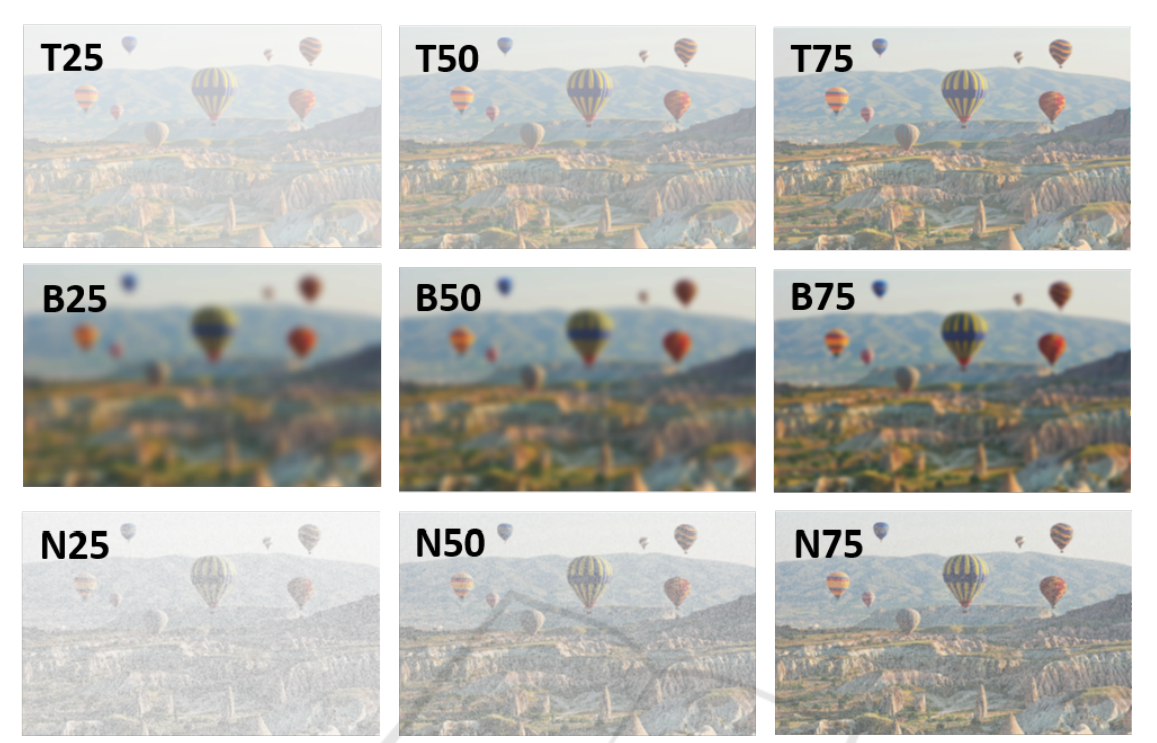
\includegraphics[width=0.9\columnwidth]{transparency-blur-noise} 
    \caption{Effetti applicati all'immagine per rendere il rischio del 25\%, 50\% e 75\%. T, B e N sono, rispettivamente, l'effetto della trasparenza, sfocatura e rumore}
\end{figure}

È stato strutturato un questionario online proposto poi a un certo numero di studenti universitari e conoscenti. I partecipanti avevano come compito quello di associare due delle 6 VV (2VV scelte casualmente per ogni effetto visivo) in due compiti di difficoltà crescente. Per tutti e due i compiti, è stato somministrato un set di riferimento a tre VV che indicavano un valore del 0\%, 50\% e 100\%, rispettivamente.\\
In questo questionario il primo compito riguardava l'accuratezza visiva (RA), il secondo compito l'accuratezza assoluta.
Nel presentare le visualizzazioni su cui si basava il questionario si ipotizzavano due possibili fonti di bias che avrebbero potuto influenzare l' analisi:
\begin{itemize}
\item l'ordine delle domande (bias di ordine);
\item il valore della percentuale mostrata (ovvero, bias di campionamento).
\end{itemize}

Per ridurre il primo tipo di bias, il questionario online è stato implementato in modo che la presentazione dei 3 effetti diversi ai partecipanti fosse in ordine casuale.\\
Le VV sono risultate utili nel comunicare probabilità sotto e sopra il 50\%, con una tendenza a sovrastimare i valori bassi e a sottostimare quelli alti. Non sono emerse differenze significative tra sfocatura, trasparenza e rumore, eccetto la trasparenza, più efficace al 40\%.\\
In particolare le visualizzazioni vaghe sono uno strumento valido per comunicare valori intermedi, mentre è stata registrata una regressione alla media quando vengono mostrati valori estremi.\\
Infine, non è stato individuato un metodo migliore di altri. Gli studiosi contano di effettuare altri esperimenti in ambienti controllati e reali per verificare se le decisioni prese dai medici sono diverse quando la previsione del rischio è rappresentata con quantità evidenti, o mediante una visualizzazione vaga. Si conta anche di misurare la soddisfazione dei medici.\\

Un altro studio interessante che utilizza le visualizzazioni vaghe è lo studio "Comparative Assessment of Two Data Visualizations to Communicate Medical Test Results Online"\footcite{womak:comparative-assesment}, dove si prendono in esame test diagnostici basati su biomarcatori, cioè indicatori di una specifica condizione, nella fattispecie l'infezione da SARS-CoV-2, causa di COVID-19.\\
Ogni test diagnostico, sia esso basato su imaging, carica virale o presenza di antigeni, è associato a un certo margine di errore, ma razionalmente tendiamo a considerare l'esito del test solo in termini di sì/no, evitando di valutare la probabilità di avere o non avere una specifica condizione. Utilizzando gli strumenti di supporto decisionale basati su ML, l'elemento probabilistico può essere reso visibile e quindi esplicitato, ad esempio riportando i punteggi di probabilità o rappresentandoli in un qualche modo: in questo studio i ricercatori ritengono che questo possa aiutare gli utenti ad interpretare al meglio l'output della macchina. In pratica l'incertezza intrinseca di questi modelli può costituire un plus nel processo decisionale, ad esempio per scegliere se sottoporsi ad un ulteriore esame o per prediligere una terapia.\\
Tale studio ha quindi lo scopo di scegliere la migliore visualizzazione dei dati da presentare agli utenti relativamente ad un test ematologico per rilevare le infezioni da COVID-19, mediante il Conteggio Ematologico Completo, utilizzando un modello di ML. Questo modello è stato convalidato nella letteratura di riferimento e poi incorporato in uno strumento basato sul Web.\\
Sono state confrontate due visualizzazioni progettate secondo i principi delle visualizzazioni vaghe: le stime incerte sono rappresentate evitando volutamente l'utilizzo dei simboli, cioè numeri e rappresentazioni metriche, come estensioni della lunghezza e angoli. Secondo le caratteristiche delle visualizzazioni vaghe, le quantità probabilistiche sono presentate come indizi visivi, i quali sono difficili da interpretare in termini razionali, cioè sono difficili da associare a valori numerici. Si utilizzano specificamente tonalità di colore o gradienti di saturazione e luminosità. Questa modalità è voluta e mira a comunicare ai lettori un senso di incertezza e vaghezza per far sì che i lettori comprendano effettivamente le stime visualizzate, come rischi, probabilità, dispersione. È evidente che le visualizzazioni vaghe richiedono una attenzione aggiuntiva.\\

Le due visualizzazioni citate sono state ideate durante due sessioni di progettazione in cui sono stati coinvolti sia gli autori di questo articolo sia i clinici che hanno sviluppato il modello statistico. I clinici sono stati adeguatamente edotti circa le caratteristiche delle visualizzazioni vaghe e sono stati invitati a co-progettare due visualizzazioni: una visualizzazione destinata a colleghi esperti nell'interpretare i test di laboratorio, e una più semplice che potesse essere più familiare ai pazienti testati.\\
Le visualizzazioni risultanti si basavano su metafore diverse: la prima visualizzazione si basava sul comune \gls{test-del-tornasole} e sulla metafora della bolla livello; la seconda visualizzazione dei dati adottava la metafora del bastoncino di test, utilizzata, ad esempio, nei test di gravidanza, e quindi familiare al pubblico in generale.
Lo studio è stato concepito per capire:\\
\begin{enumerate}
    \item se la metafora del bastoncino di test fosse adeguata in caso di una risposta sensibile e delicata
    come quella relativa alla positività al COVID-19, o, come osservato in alcuni studi, finisse per
    confondere troppo spesso le persone comuni
    \item se una visualizzazione dei dati più tecnica, quella progettata per gli operatori sanitari, potesse
    essere comprensibile anche al pubblico comune.
\end{enumerate}
Nella visualizzazione a bolla livello, il risultato del test è presentato attraverso la posizione di una bolla circolare all'interno di una barra a tre colori (simile al tornasole). Si valuta quindi la sua maggiore o minore vicinanza a uno degli estremi della barra per indicare una condizione COVID-19-positiva o negativa (rispettivamente all'estremo rosso più a sinistra e all'estremo blu più a destra). I risultati incerti, cioè quelli a bassa affidabilità, sono caratterizzati da una sostanziale equidistanza della bolla dagli estremi, corrispondente ad un posizionamento nella zona grigia centrale della barra tornasole. L'incertezza è anche resa evidente dalla dimensione della bolla: più grande è la bolla, maggiore è l'intervallo di confidenza della stima della probabilità.\\

\begin{figure}[!ht] 
    \centering 
    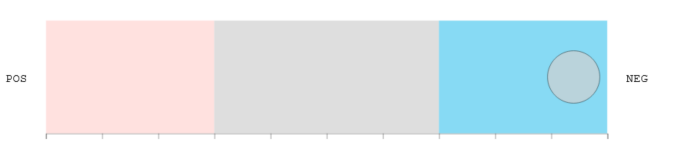
\includegraphics[width=0.9\columnwidth]{metafora-bolla} 
    \caption{Natura dell'incertezza}
\end{figure}

\begin{figure}[!ht] 
    \centering 
    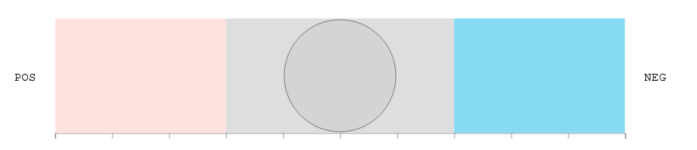
\includegraphics[width=0.9\columnwidth]{metafora-bolla-2} 
    \caption{Natura dell'incertezza}
\end{figure}

La visualizzazione del bastoncino di test fornisce le medesime informazioni visualizzate tramite la bolla livello, ma attraverso affordance (in senso generale, favorire l'utilizzo) e segnali visivi diversi.\\
Nel dettaglio si vedono due fasce rosse: una per indicare l'affidabilità della risposta e indicata con una C maiuscola ("controllo"), e una che indica il risultato del test, indicata con un segno più singolo (+). In pratica questa visualizzazione restituisce l'output del modello in termini di opacità della barra: più trasparenti (e meno visibili) sono la fascia + e la fascia C, minore è la probabilità che il test sia associato a una condizione positiva e che il test sia affidabile. Un test quasi certamente negativo è quindi reso da un bastoncino in cui è chiaramente visibile solo la barra C,mentre un test non valido è rappresentato da un bastoncino in cui nessuna fascia rossa è  visibile.\\

In conseguenza dei risultati positivi riscontrati nei due studi sopra citati, è nata l'idea di utilizzare lo stesso tipo di comunicazione dell'incertezza nel progetto Epimetheus.
